\subsection{Experiment Setup}
\label{sec:preprocess}
In this paper, we use Probase\cite{WuLWZ12} and WordNet\cite{wordnet}
as two alternative isA taxonomies.
Consequently, we build two lexicons, one
for Probase and one for WordNet. Probase is a large collection of
concept-subconcept or concept-entity pairs which were
extracted automatically
%by the Hearst pattern\cite{Hearst92}
from a large web corpus.
%Because this knowledge base is harnessed from large data,
It contains statistical scores of the extracted pairs,
such as the popularity,
and the conditional probability between the concept and its sub-concept.
WordNet, on the other hand, is a smaller, cleaner knowledge base manually
curated by experts and does not contain any scoring information.
These two taxonomies provide two different vocabularies of concepts
from which to draw the solution of AC.
%Our primary target of verb is a set of 200 most frequently used verbs in
%English text\footnote{We compute the frequency of all verbs that appeared
%in a very large web text corpus to obtain the 200 most frequently used
%verbs. We excluded a few verbs such as ``use'', ``make'', ``get'' and
%``take'' from the top of the list because they are extremely general and
%have too many arguments.},
%which we call Verb-200. These verbs are shown in \figref{fig:verbs}. A random
%sample of 20 verbs from Verb-200 forms a smaller set of verbs called Verb-20
%(highlighted in \figref{fig:verbs}) which are used in most of our experiments.

%All our experiments are based on two large
%datasets\footnote{We release most of
%our datasets and the action concept lexicon at
%\url{http://202.120.38.146/~kzhu/ac}.}
%from Web sentences (called Web for short) and
All action instances we use in this work come
from the {\em Verbargs} package of Google syntactic N-gram
data\cite{goldberg2013,googlengram} (called Google for short).
%respectively. The Web dataset contains 49,911,718 verb-subject pairs
%and 65,035,827 verb-object pairs extracted from 165,758,215 English
%sentences, which is a crawled snapshot of web pages.
The data set, which was extracted by parsing millions of books,
contains 32,731,395 verb-subject and 
43,580,062 verb-object relations.\footnote{We focus on verb-subject and
verb-object relations in this work while
other kinds of action instances can also be used.}
From these relations, we obtain 10,116 English verbs or verb phrases as well as
their relations after filtering out obvious errors and low frequency verbs.
Among these, 8219 are single word verbs, 1888 are two-word verb phrases, and
9 are three-word verb phrases.
These form the target set of verbs (known as {\bf Verb-10k}) for 
the lexicon construction.  These verbs not only cover more than 
90\% of those verbs (3096 of them) in FrameNet 1.5,
but also include many other commonly used terms. 
A random sample of those verbs in Verb-10k but {\em not} in
FrameNet is shown in \figref{fig:verb10k}. 
We further randomly sample 20 verbs
by frequency from Verb-10k to form a smaller development set called 
{\bf Verb-20},
shown in \figref{fig:verb20}. These are more frequently 
used verbs with many action instances.
%from the \emph{Verbargs} package, which includes 130,436,458
%syntactic N-grams.
% with verb-argument dependencies.
%\KZ{How many subject-verb pairs and verb-object pairs in google data?}
%\KZ{Kaiqi: We need to describe how we generate the web and
%google data sets here.
%Need to emphasize how big these data sets. Remember this ``VL''DB!}

%We build our action lexicon based on two verb sets extracted from
%the two datasets. The 3734 most frequently used verbs (including verb phrases)
%in the Web data form a primary verb set called {\bf Verb-3734}.
%A subset of 2323 verbs that can be found in the Google dataset
%form the other verb set called {\bf Verb-2323}. \KQ{These verbs cover
%more than 99\% of sentences/n-grams in the two datasets, respectively.
%%We compute the frequency of all verbs that appeared
%%in a very large web text corpus to obtain the 3734 most frequently used
%%verbs.
%We also randomly sample 20 verbs from the 200 most frequently
%used verbs to form another small set of verbs called {\bf Verb-20}
%(in \figref{fig:verb20}) %which are used in most of our experiments.
%for human evaluation on some experiments, because it is expensive
%to label for all verbs in Verb-3734 and Verb-2323.}
\begin{figure}[th]
\centering
\fbox{\parbox{.8\columnwidth}{
averse,
blossom,
blush,
calculate,
center,
commercialize,
contort,
cut back,
demonize,
disclaim,
drain out,
electrify,
filter out,
hydrolyze,
lead away,
line up,
lure,
oversee,
preprocess,
recapture,
reenforce,
reprise,
round out,
skim off,
touch up,
typeset
}}
\caption{Samples from Verb-10k but not in FrameNet}
\label{fig:verb10k}
\end{figure}


\begin{figure}[th]
\centering
\fbox{\parbox{.8\columnwidth}{
bring,
carry,
connect,
cut,
define,
eat,
help,
hit,
keep,
operate,
perform,
play,
read,
release,
report,
select,
spend,
submit,
visit,
wear
}}
\caption{Verbs in Verb-20}
\label{fig:verb20}
\end{figure}

ReVerb also provides millions of relation triples, some of which contain
verbs as predicate.
%However, the scale of ReVerb is small to our problem.
We aim at discovering the action concepts,
which needs a large number of action instances
for each verb. However, ReVerb contains small number of triples for each verb.
For example, only 374 unique triples for ``wear'' are
extracted in ReVerb while our web dataset contains 17,749 unique
\pair{verb}{object} pairs for ``wear''.
The reason of the huge different is that,
a triple must contain two arguments for the verb in ReVerb. However,
verbs co-occur with only one argument in many cases.
Moreover, ReVerb has little coverage on
intransitive verbs, which only come with subject.
We give up using ReVerb data due to these limitations.
%\KZ{We need to explain why we don't use the ReVerb data.}

%\subsection{Preprocessing of Dataset}
%To make use of the web sentences and Google syntactic N-gram,
%Next, we preprocess the two datasets as follows to
%generate action instances.
%
%{\bf Web} data comes from the result of Stanford dependency parser,
%%We run a dependency parser on the whole corpus and
%which are dependency trees for the sentences. We are interested in
%verb-subject and verb-object relations only.
%The head word of subject is usually labeled
%as ``nsubj'' or ``agent'' while the head word of object is usually
%labeled as ``dobj'' or ``nsubjpass''.
%We can retrieve the entire phrase of subject or object in the dependency
%tree by returning the whole subtree rooted on the head.
%However, the whole phrase of subject/object is not always
%a term recognizable by the taxonomies. As shown in \figref{fig:pterm},
%the phrase ``a flashy baseball cap''
%is extracted as the object of ``wear'', but
%it is not a valid Probase/WordNet term.
%To make use of the taxonomies, we need to
%detect the Probase/WordNet term from the subject/object phrase
%(e.g., baseball cap).
%
%\begin{figure}[th]
%\centering
%\epsfig{file=pterm.eps,width=0.8\columnwidth}
%\caption{Dependency Parse Tree}
%\label{fig:pterm}
%\end{figure}
%
%We use a sliding window strategy to extract longest
%Probase/WordNet term that we can detect in the whole phrase.
%The window slides around the head word
%from right to left, and check if a Probase/WordNet term exists.
%The initial size of the window is the length of the
%whole phrase. If we detect a Probase/WordNet term,
%we return the phrase captured in the window;
%Otherwise, we decrease the window size and slides
%around the head term again. We stop until we find
%any Probase/WordNet term. Usually, this procedure can detect
%a Probase/WordNet term from the phrase, because Probase/WordNet includes
%most of the words (phrase with length 1). After
%preprocessing, we output all the pairs of verb-subject and
%verb-object as action instances.
%%\begin{table}[th]
%%\centering
%%%\scriptsize
%%\caption{Snapshot of Google Syntactic N-gram}
%%\begin{tabular}{|l|l|}
%%\hline
%%Verb & N-gram \\
%%\hline \hline
%%accept & firms/NNS/nsubj/2\; accept/VBP/conj/0\; \\
%%& money/NN/dobj/2\; in/IN/prep/2\; \\
%%& exchange/NN/pobj/4   \\
%%\hline
%%delay & to/TO/aux/2\; delay/VB/xcomp/0\; \\
%%& these/DT/det/4\; matters/NNS/dobj/2 \\
%%\hline
%%spent & an/DT/det/2\; afternoon/NN/nsubjpass/4\; \\
%%& was/VBD/aux/4\; spent/VBN/conj/0\\
%%\hline
%%\end{tabular}
%%\label{tab:ngram}
%%\end{table}

%\textbf{Google} data contains relations between
%verbs and arguments.
%A snapshot
%of Google syntactic n-gram is shown in \tabref{tab:ngram}.
%The syntactic n-gram consist of the dependency parsing
%result conducted by Stanford parser.
%\KZ{Do we still need the following??}

In the Google data, each token is labeled with POS tag and dependency, 
and thus each ngram is represented by a dependency tree.
We extract pairs of \pair{verb}{subject} and \pair{verb}{object}
from the dependency tree according to subject-verb dependency (nsubj, 
agent) and object-verb dependency (dobj, nsubjpass).
Since the dependency only specifies the head word of subject/object,
to extract the whole subject/object phrase in the dependency tree, we 
retrieve the subtree rooted on the head word to construct a candidate
subject/object phrase. In order to make use of the knowledge bases, 
the subject/object phrases should be recognized by Probase/WordNet.
Thus, we use a sliding window on the candidate phrase to further 
extract the most probable (longest) Probase/WordNet term. 

%First, we restore each n-gram to a dependency tree
%according to the head index. Next, we find the head of the
%subject or object from the nodes that directly connects to
%the verb node with a dependency label such as ``nsubj'', ``agent'', ``dobj''
%or ``nsubjpass''. Around the head, we use the same sliding window
%algorithm to find a longest Probase/WordNet term to be the subject/object
%as in the processing of the web data. Also, we convert
%the verb to its lemma form.
%After this process, we finally get two lists of pairs
%in the form of \pair{verb}{subject} and \pair{verb}{object}, respectively.

%The subsequent experiments are conducted on lexicons learned from
%different combinations of verb sets, taxonomies and datasets. For
%readers' convenience, the configurations of these experiments are documented
%in \tabref{tab:comb}. \KQ{Among these experiments, accuracy \& overlap and
%argument identification need human annotations so that we conduct these
%two experiments on the small verb set. We use the lexicon learned using
%WordNet in verb sense matching and WSD because we need to
%compare with WordNet classes in evaluation. The other experiments
%are based on Probase and Web, which is our default configuration.
%The value of $\tau$ is set to $0.2$, which achieves the most accurate lexicon.
%}
%
%\begin{table}[th]
%\centering
%\scriptsize
%\caption{Verbs, taxonomies and datasets for each experiment}
%\begin{tabular}{|l|c|c|c|}
%\hline
%Experiment & Verb Sets & Taxonomies & Datasets \\
%\hline \hline
%Accuracy \& Overlap & Verb-20 & Probase &  Web, Google\\
%\hline
%\multirow{2}{*}{Execution Times} & Verb-3734, & Probase,
%	& \multirow{2}{*}{Web, Google} \\
%	& Verb-2323 & WordNet & \\
%\hline
%Verb Sense Matching & Verb-3734 & WordNet & Web \\
%\hline
%Argument Identification & Verb-20 & Probase & Web \\
%\hline
%WSD & Verb-3734 & WordNet & Web \\
%\hline
%Verb Frame Generation & Verb-3734 & Probase & Web \\
%\hline
%Term Similarity & Verb-3734 & Probase & Web \\
%\hline
%\end{tabular}
%\label{tab:comb}
%\end{table}
%
%\begin{figure}[th]
%\centering
%\fbox{\parbox{2\columnwidth}{
%\sout{use
%make
%include
%take
%get
%provide
%show}
%go
%say
%find
%see
%come
%work
%need
%look
%require
%give
%{\bf help}
%offer
%know
%create
%change
%add
%start
%allow
%{\bf keep}
%{\bf play}
%contain
%run
%apply
%receive
%call
%develop
%leave
%begin
%hold
%support
%cause
%build
%meet
%increase
%cover
%base
%want
%serve
%continue
%{\bf read}
%write
%produce
%{\bf bring}
%involve
%pay
%live
%ask
%put
%consider
%set
%reduce
%remove
%improve
%appear
%{\bf perform}
%seem
%move
%lead
%follow
%buy
%occur
%try
%design
%contact
%complete
%sell
%learn
%determine
%think
%{\bf report}
%describe
%like
%present
%mean
%relate
%lose
%feel
%affect
%post
%represent
%enjoy
%send
%open
%discuss
%{\bf visit}
%enter
%grow
%share
%maintain
%identify
%indicate
%tell
%place
%list
%return
%choose
%{\bf select}
%turn
%sign-up
%form
%obtain
%stop
%check
%result
%win
%happen
%install
%{\bf wear}
%die
%love
%understand
%save
%expect
%focus
%fill
%watch
%prevent
%{\bf spend}
%protect
%reach
%pass
%raise
%display
%treat
%ensure
%{\bf connect}
%achieve
%establish
%suggest
%view
%accept
%associate
%fit
%drive
%exist
%control
%talk
%replace
%deliver
%avoid
%hear
%fall
%let
%{\bf define}
%handle
%{\bf eat}
%plan
%bear
%prepare
%manage
%{\bf release}
%promote
%attend
%experience
%join
%kill
%seek
%{\bf operate}
%measure
%end
%refer
%teach
%face
%conduct
%explain
%purchase
%combine
%test
%{\bf cut}
%generate
%review
%deal
%break
%close
%reflect
%decide
%believe
%consist
%{\bf carry}
%fail
%collect
%speak
%address
%encourage
%match
%stand
%sit
%stay
%{\bf hit}
%{\bf submit}
%draw
%walk
%depend
%limit
%please
%reveal
%introduce
%wait
%arrive
%enable
%}}
%\caption{Verb-200 (Ranked) with Verb-20 in Bold}
%\label{fig:verbs}
%\end{figure}

%bring\\
%carry\\
%connect\\
%cut\\
%define\\
%eat\\
%help\\
%hit\\
%keep\\
%operate\\
%perform\\
%play\\
%read\\
%release\\
%report\\
%select\\
%spend\\
%submit\\
%visit\\
%wear\\
%\hline
%\end{tabular}
%\label{tab:verbs}
%\end{table}
%


